\documentclass[a4paper,10pt]{article}

\usepackage[utf8]{inputenc}
\usepackage[spanish]{babel}
\usepackage{multicol}
\usepackage{blindtext}
\setlength{\parindent}{0pt}
\setlength{\columnsep}{1cm}
\usepackage{anysize}
\marginsize{2.75cm}{2.75cm}{1.5cm}{1.5cm}
\usepackage[pdftex]{graphicx}
\usepackage{float}
\usepackage{amsmath}

\begin{document}

\title{Quantum Chromodynamics and \\ Quantum Computation and Simulation}
\author{Juan José Gálvez Viruet}
\date{\today}
\maketitle

\begin{abstract}
\noindent URL: https://github.com/jjgalvezviruet/Proyecto\_Final\_GitLatex

Gracias al rápido desarrollo experimental de las <<tecnologías cuánticas>> se ha hecho posible la construcción de sistemas, como las redes de iones, los semiconductores o las <<optical lattices>>, en los que las interacciones entre sus componentes se pueden controlar de manera muy precisa. Estas interacciones vienen descritas por la mecánica cuántica, por lo que los sistemas en su conjunto ofrecen diversas oportunidades para estudiar efectos cuánticos, como el entrelazamiento, en áreas como la computación o la simulación.

Entre los diversos campos que pueden beneficiarse del desarrollo de estas tecnologías esta la física de partículas, donde sus componentes interacciones de maneras muy diversas, todas descritas por teorías cuánticas de campos basadas en algún grupo de simetría gauge. La Cromodinámica Cuántica (QCD) es la teoría de la interacción fuerte, encargada de mantener al núcleo atómico unido, y su estudio es fundamental para entender la fenomenología del Modelo Estándar y la comprensión de los primeros instantes del cosmos. Debido a su complejidad no puede abordarse desde una única perspectiva y se trabaja o bien con teoría de perturbaciones para caracterizar su régimen de altas energías o bien con simulaciones clásicas basadas en métodos Monte Carlo para fenómenos a bajas energías. A continuación nos centraremos en definir los límites de la computación clásica y en mostrar a las nuevas tecnologías cuánticas como posibles vías para superarlos.

Palabras clave: \textit{Quantum computation, quantum simualtion, lattice gauge theories, QCD}
\end{abstract}

\begin{multicols}{2}
\section{Introducción} 
Las teorías cuánticas de campos con simetría gauge (o teorías gauge) son la base sobre la que se construye el Modelo Estándar de partículas \cite{Peskin:1995ev}. Su expresión más fundamental se da en forma de funciones Lagrangianas o Hamiltonianas, con términos cinéticos y de interacción construidos de tal manera que se respeta cierto tipo de transformación llamada simetría gauge. Las teorías gauge que describen las interacciones fundamentales electromagnética (Electrodinámica Cuántica, QED) y fuerte (Cromodinámica Cuántica, QCD) son especialmente importantes y se basan en los grupos de simetría (abeliano) U(1) y (no abeliano) SU(3).

El cambio en la intensidad de las interacciones con la escala de energía es una de las características más importantes de las teorías cuánticas de campos: Para teoría abelianas como QED la interacción puede tratarse como una pequeña perturbación a la dinámica libre de las partículas hasta escalas de energía medias y bajas; para teorías no abelianas como QCD el régimen perturbativo es válido solo a altas energías, mientras que a medias y bajas energías la matería está interaccionea muy intensamente, propiedad a la que se denomina \textit{libertad asintótica}.

La libertad asintótica de QCD impide el uso de métodos perturbativos para el estudio de cualquier proceso dinámico entre partículas que interacciones a bajas y medias energías, como por ejemplo la formación y dinámica de protones, neutrones y otros hadrones. En estos casos se usa un enfoque distinto denominado \textit{Lattice QCD} \cite{particle_data_group_review_2018}, que consiste en la codificación de los grados de libertad de la teoría en una red de puntos (para la materia) y conexiones (para las interacciones), que permite generar todas las posibles configuraciones que se dan en un proceso, con las que se obtienen obervables físicos relevantes mediante un posterior análisis estadístico. 

Las configuraciones de la red se generan siguiendo una distribución de probabilidad que se obtiene a partir del Lagrangiano de la teoría mediante un método denominado \textit{importance sampling}, por el que solo se generan los estados más probables. Su principal limitación viene asociada a errores estadísticos, causados por la dificultad de reproducir la distribución de probabilidad del sistema y sistemáticos, que vienen a su vez de la discretización. Estos errores se vuelven difíciles de controlar cuando se quiere estudiar la dinámica de partículas pesadas, mientras que muchos procesos dinámicos quedan fuera de su alcance debido al ``problema del signo'' \cite{particle_data_group_review_2018,usqcd_collaboration_hot-dense_2019}. 

Estas limitaciones son inherentes al uso de métodos de generación de distribuciones de probabilidad clásicos y ya fue señalado por Feynman \cite{feynman_simulating_1982} como una de las posibles razones para el desarrollo de computadores basados en las leyes de la mecánica cuántica, que hoy en día empiezan a ser una realidad con la que se espera superar las barreras actuales.

\section{El diagrama de fases de QCD}
Uno de los objetivos de investigación a largo plazo de la comunidad de física nuclear y de altas energías es la exploración del diagrama de fases de la materia que interacciona fuertemente (figura \ref{QCDphase}). Fruto de esta investigación se ha descubierto por ejemplo que la transición entre la materia hadrónica (estados compuestos en QCD) y la fase de plasma de quarks y gluones a bajo potencial químico es continua, mientras que se sospecha que a valores más altos de este si que ocurra una transición de fase con un punto crítico.

\begin{figure}[H]
\begin{center}
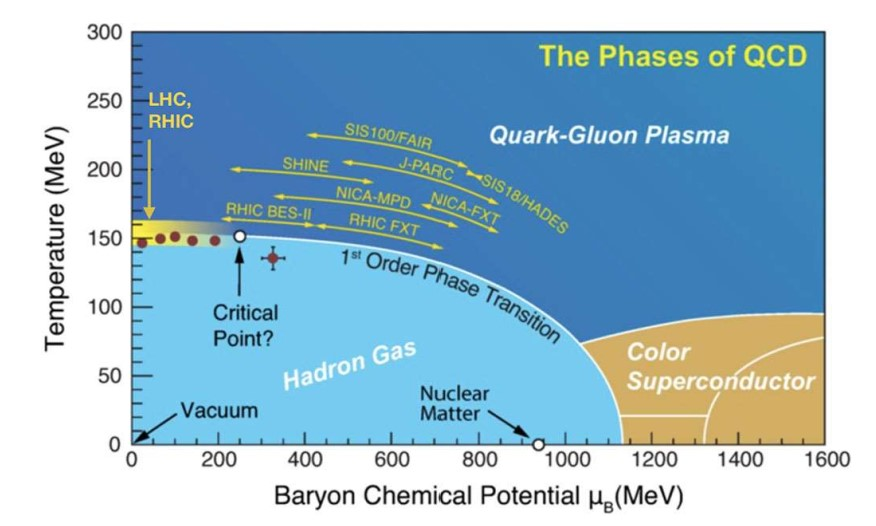
\includegraphics[scale=0.6]{Imágenes/DiagramaQCD.jpg}
\end{center}
\caption{Diagrama de fases de QCD, podemos apreciar tres regiones: el plasma de quarks y gluones (QGP), el gas de hadrones y una fase superconductora. Figura extraída de \cite{usqcd_collaboration_hot-dense_2019}}
\label{QCDphase}
\end{figure}

Conocer el diagrama de QCD, y en especial la parte correspondiente al plasma de quarks y gluones, es importante porque se supone que esta fue la fase de la materia en los primeros instantes del universo y se cree que podría ser el material del que están compuestos los núcleos de las estrellas de neutrones \cite{busza_heavy_2018}.

Los métodos basados en lattice son aplcicables en la región con potencial químico ($\mu$) igual a cero, es decir, con igual número de partículas y antipartículas y aunque existen vías de ampliarlos para abarcar la región cercana al eje $\mu=0$ \cite{usqcd_collaboration_hot-dense_2019}, el estudio de la dinámica de la materia nuclear y de la posible fase superconductora esta fuera de su alcance.

\section{Computación y simulación cuánticas}
En la sección anterior hemos presentado un ámbito en el que la computación clásica se enfrenta a imporatantes limitaciones. Una forma de superarlas, o evitarlas, es el uso de sistemas gobernados por las leyes de la mecánica cuántica para simular otros sistemas a su vez gobernados por las mismas leyes. Entre el ``hardware'' más prometedor para conseguir este obetivo están las trampas de iones, la manipulación de fotones, los superconductores y los sólidos dopados \cite{ladd_quantum_2010}.

Existen dos formas de construir estos simuladores: la simulación digital partiría de un sistema en el que se han implementado ciertas puertas lógicas cuánticas que permitirían la evaluación de cualquier expresión, mientras que en los simuladores analógicos dicha evolución se conseguiría directamente a través del ``hardware'', que estaría construido especificamente para esa tarea \cite{cirac_goals_2012}.

Dado que aún no se posee una computadora cuántica lo suficientemente potente como para implementar en ella una teoría de gauge, los primeros trabajos en este sentido han usado la simulación analógica. En \cite{martinez_real-time_2016} se consigue implemetar el Hamiltoniano de QED en 1 dimensión (modelo de Schwinger) 
\begin{align*}
\hat{H}_{lat} &  = -iw\sum_{n=1}^{N-1}\left[\hat{\Phi}^{\dagger}_{n}e^{i\hat{\theta}_{n}}\hat{\Phi}_{n+1} \right] \\
 + & J\sum_{n=1}^{N-1}\hat{L}_{n}^2 + m \sum_{n=1}^{N}(-1)^{n}\hat{\Phi}^{\dagger}_{n}\hat{\Phi}_{n},
\end{align*}
donde el segundo término representa la energía del ``campo eléctrico'', el tercero la energía necesaria para crear un par electrón (partícula) positrón (antipartícula) y el primero la energía cinética de los electrones y positrones, que varía según el campo eléctrico debido al término $e^{i\hat{\theta}_{n}}$. En el estudio este Hamiltoniano se implementa en una red de cuatro iones cuyos acoplamientos se controlan por medio de pulsos láser globales e individuales (en \cite{davoudi_towards_2020} se puede encontrar una descripción más detallada de este proceso), de modo que la evolución temporal de los estos iones emula la del modelo de Schwinger, la figura \ref{SchwingerDensity} compara la densidad de partículas medida en la simulación con el resultado analítico. 
\begin{figure}[H]
\begin{center}
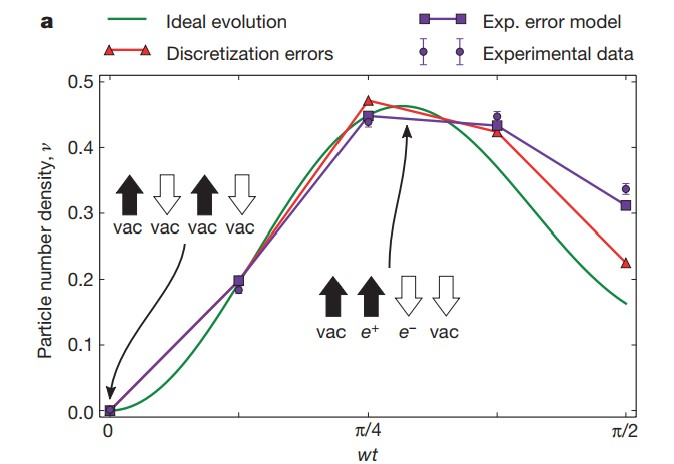
\includegraphics[scale=0.8]{Imágenes/Creación pares partícula-antipartícula.jpg}
\end{center}
\caption{Evolución de la densidad de partículas partiendo del estado fundamental (vacío) de la teoría de Schwinger mediante cálculo analítico (línea verde) y simulación en una red de cuatro iones (puntos morados). El estado del sistema se codifica mediate el espín de los iones, siendo espín ``hacia arriba'' en posiciones impares el vacío y en posiciones pares un positron, mientras que espín ``hacia abajo'' en posiciones pares indica el vacío y en posiciones impares un electrón.}
\label{SchwingerDensity}
\end{figure}

El artículo \cite{martinez_real-time_2016}, aunque este lejos de reproducir resultados que puedan competir con las herramientas usadas en la actualidad, muestra que la simulación cuántica de teorías gauge es posible. Numerosos trabajos se centran ahora en ampliar el alcance de estas simulaciones a teorías más complejas en más de una dimensión \cite{davoudi_towards_2020,paulson_towards_2021} y en desarrollar métodos generales para el uso de la computación cuántica en las teorías gauge \cite{banuls_simulating_2020,kan_lattice_2022}

\section{Conclusions}
A modo de conclusiones presentamos una tabla comparativa entre los métodos de simulación clásicos y los métodos de computación emergentes basados en tecnologías cuánticas.

\begin{tabular}{c|c}
Computación Clásica & Tecnologías cuánticas \\
\hline
\begin{minipage}{0.2\textwidth}
\begin{enumerate}
\item Maduras y conocida
\item Con resultados importantes
\item Situaciones estáticas
\end{enumerate}
\end{minipage}

&

\begin{minipage}{0.2\textwidth}
\begin{enumerate}
\item En desarrollo
\item Demostrada para sistemas sencillos
\item Situaciones dinámicas
\end{enumerate}
\end{minipage}

\end{tabular}


\begin{tabular}{c|c}
Computación Clásica & Tecnologías cuánticas \\
\hline
\begin{minipage}{0.2\textwidth}
\begin{enumerate}
\item[$4$] Basado en Lagrangiano
\item[$5$] Inadecuada para sistemas cuánticos complejos
\end{enumerate}
\end{minipage}

&

\begin{minipage}{0.2\textwidth}
\begin{enumerate}
\item[$4$] Basado en Hamiltoniano
\item[$5$] Pensada para estudiar la dinámica cuántica
\end{enumerate}
\end{minipage}

\end{tabular}

\bibliography{QCD&QComputation}
\bibliographystyle{naturemag}
\end{multicols}


\end{document}